\documentclass[twocolumn,longbibliography]{revtex4-1}
\usepackage{hyperref}
\usepackage{verbatim}
\usepackage[imagemagick]{sagetex}
%can be removed only for testing
\usepackage{lipsum}
\setlength{\sagetexindent}{10ex}

\begin{document}
\bibliographystyle{plain}%Choose a bibliograhpic style
\title{Algebraic geometry to solve machine learning problems}
\author{G. R. Sasikanth}
\email{sraghava@gunaatita.com}
\homepage{https://darkcornerlaboratory.wordpress.com/}
\affiliation{Gunaatita technologies, Data Science Research - India}
\date{\today}
\keywords{Machine Learning, Algebraic Geometry, Elastica, Euler Spiral}
\begin{abstract}
 In this article, we briefly describe various tools and approaches that algebraic geometry has to offer to straighten bent objects.
 throughout this article we will consider a specific example of a bent or curved piece of paper which in our case acts very much like an     
 elastica curve. We generalize this model to various shapes of paper which are stretched and bent and then finally implement it on 
 a standard 80mg paper and see how the folds on paper can be completely removed using python and sage-math code. We conclude this article
 with a suggestion to algebraic geoemtry as a viable and fast performant alternative of neural networks in vision and
 machine learning.The purpose of this article is not to build a full blown framework but to show evidence or possibility of using 
 algebraic goemetry as an alternative to recognizing or extracting features on manifolds.
\end{abstract}
\maketitle

\section{Introduction}
Elliptic curves and curves from algebraic geometry have surfaced many times in the recent years in fields related to computer vision ~\cite{Mumford} and machine learning. Mumford has succesfully demonstrated that elastica curves can be represented as the curve that maximizes the likelihood of a random curvature variable.Levin has made a detailed historical report of these curves in detail ~\cite{Levien} .While most of the applications have been indirect in nature in this article we tried to find a direct application to
elastica curves and euler spirals.In computer vision modifying the a scanned document to a shape that is geometrically flat is a much sort out problem. Very effective solutions already exist that can deskew ,rotate and liearize. While most of them are supervised approaches that require a large data sets before we can straighten the document.In this article we try to build a solution that strictly involves geometric modelling of the surface of a paper without requiring to use any supervised machine learning techniques.These appliations can be very useful in deflattening the surface of a scanned document attached to a book using a handheld device like mobile phone. This approach can be usedvery effectively to convert the curved graphics on the centere fold end of a book which are often very difficult to read from a scanned pdf file. Mobile applications like office lens and cam scanner can use this application to make the scanned view more readable without putting too mcuh stress on resource crunched mobile phones.

\section{Problem Statement}
when a book is opened there is a certain curvature that surfaces of the pages forms, the corners of the pages are usually curved and is often difficult to read the inners parts of .It becomes even harder to read the pages when if it is a document scanned from a book with lot of pages. The curvature of the document is shown in a side view in figure 1. The problem is to identify the curve in figure 1 and use computational technques to geometrically flatten the scanned documents .
\begin{figure*}
  \centering
  \caption{OpenBook}
  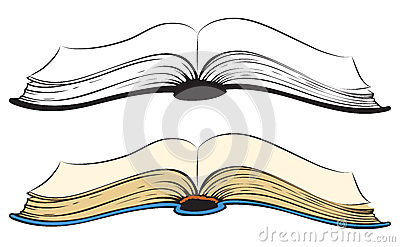
\includegraphics[scale=5]{figure1.jpg} 
\end{figure*}

\section{Proposed Solution}


\bibliography{Master}
\end{document}

